\ifx\wholebook\relax \else

\documentclass{article}

%
% loading packages
%

\RequirePackage{ifpdf}
\RequirePackage{ifxetex}

%
%
\ifpdf
  \RequirePackage[pdftex,%
       bookmarksnumbered,%
              colorlinks,%
          linkcolor=blue,%
              hyperindex,%
        plainpages=false,%
       pdfstartview=FitH]{hyperref}
\else\ifxetex
  \RequirePackage[bookmarksnumbered,%
               colorlinks,%
           linkcolor=blue,%
               hyperindex,%
         plainpages=false,%
        pdfstartview=FitH]{hyperref}
\else
  \RequirePackage[dvipdfm,%
        bookmarksnumbered,%
               colorlinks,%
           linkcolor=blue,%
               hyperindex,%
         plainpages=false,%
        pdfstartview=FitH]{hyperref}
\fi\fi
%\usepackage{hyperref}

% other packages
%--------------------------------------------------------------------------
\usepackage{graphicx, color}
\usepackage{wrapfig}
\usepackage{subfig}
\usepackage{multicol}
\usepackage{tikz}
\usetikzlibrary{matrix,positioning,shapes}
\usetikzlibrary{patterns}

\usepackage{amsmath, amsthm, amssymb} % for math
\usepackage{exercise} % for exercise
\usepackage{import} % for nested input

%
% for programming
%
\usepackage{verbatim}
\usepackage{fancyvrb}
\usepackage{listings}
%\usepackage{algorithmic} %old version; we can use algorithmicx instead
%\usepackage[plain]{algorithm} %remove rule (horizontal line on top/below the algorithm
\usepackage{algorithm} %to remove rules change to \usepackage[plain]{algorithm}
%\usepackage{algorithm2e}
\usepackage[noend]{algpseudocode} %for pseudo code, include algorithmicsx automatically
\usepackage{appendix}
\usepackage{makeidx} % for index support
\usepackage{titlesec}
\usepackage{epigraph}

\usepackage[cm-default]{fontspec}
\usepackage{xunicode}
%\usepackage{fontenc}
\usepackage{textcomp}
\usepackage{url}

% detect and select Chinese font
% ------------------------------
% fc-list :lang=zh    % list all Chinese fonts
% fc-list :mono       % list all mono fonts
% fc-cache            % refresh cache to load new installed fonts
\def\macmainfont{STSong}  % Under Mac OS X
\def\macmonofont{Monaco}
\def\winmainfont{SimSun} % Under Windows
\def\winmonofont{Consolas}
\def\linuxmainfont{WenQuanYi Micro Hei} % Under Linux
\def\linuxmainfont{Courier}

\suppressfontnotfounderror1 % Avoid setting exit code (error level) to break make process
\count255=\interactionmode
\batchmode

% main font
\let\mainft=\macmainfont
\font\thefont="\mainft"\space at 10pt
\ifx\thefont\nullfont
  \let\mainft=\winmainfont
  \font\thefont="\mainft"\space at 10pt
  \ifx\the\nullfont
    \let\mainft=\linuxmainfont
    \font\thefont="\mainft"\space at 10pt
    \ifx\the\nullfont
      \errorstopmode
      \errmessage{no suitable Chinese main font found}
    \fi
  \fi
\fi

% mono font
\let\monoft=\macmonofont
\font\thefont="\monoft"\space at 10pt
\ifx\thefont\nullfont
  \let\monoft=\winmonofont
  \font\thefont="\monoft"\space at 10pt
  \ifx\the\nullfont
    \let\monoft=\linuxmonofont
    \font\thefont="\monoft"\space at 10pt
    \ifx\the\nullfont
      \errorstopmode
      \errmessage{no suitable mono font found}
    \fi
  \fi
\fi

\interactionmode=\count255

\setmainfont[Mapping=tex-text]{\mainft}
\setmonofont[Scale=MatchLowercase]{\monoft}   % 英文等宽字体

\XeTeXlinebreaklocale "zh"  % to solve the line breaking issue
\XeTeXlinebreakskip = 0pt plus 1pt minus 0.1pt

\titleformat{\paragraph}
{\normalfont\normalsize\bfseries}{\theparagraph}{1em}{}
\titlespacing*{\paragraph}
{0pt}{3.25ex plus 1ex minus .2ex}{1.5ex plus .2ex}

\lstdefinelanguage{Smalltalk}{
  morekeywords={self,super,true,false,nil,thisContext}, % This is overkill
  morestring=[d]',
  morecomment=[s]{"}{"},
  alsoletter={\#:},
  escapechar={!},
  literate=
    {BANG}{!}1
    {UNDERSCORE}{\_}1
    {\\st}{Smalltalk}9 % convenience -- in case \st occurs in code
    % {'}{{\textquotesingle}}1 % replaced by upquote=true in \lstset
    {_}{{$\leftarrow$}}1
    {>>>}{{\sep}}1
    {^}{{$\uparrow$}}1
    {~}{{$\sim$}}1
    {-}{{\sf -\hspace{-0.13em}-}}1  % the goal is to make - the same width as +
    %{+}{\raisebox{0.08ex}{+}}1		% and to raise + off the baseline to match -
    {-->}{{\quad$\longrightarrow$\quad}}3
	, % Don't forget the comma at the end!
  tabsize=2
}[keywords,comments,strings]

% for literate Haskell code
\lstdefinestyle{Haskell}{
  flexiblecolumns=false,
  basewidth={0.5em,0.45em},
  morecomment=[l]--,
  literate={+}{{$+$}}1 {/}{{$/$}}1 {*}{{$*$}}1 {=}{{$=$}}1
           {>}{{$>$}}1 {<}{{$<$}}1 {\\}{{$\lambda$}}1
           {\\\\}{{\char`\\\char`\\}}1
           {->}{{$\rightarrow$}}2 {>=}{{$\geq$}}2 {<-}{{$\leftarrow$}}2
           {<=}{{$\leq$}}2 {=>}{{$\Rightarrow$}}2
           {\ .}{{$\circ$}}2 {\ .\ }{{$\circ$}}2
           {>>}{{>>}}2 {>>=}{{>>=}}2
           {|}{{$\mid$}}1
}

% "define" Scala
\lstdefinelanguage{Scala}{
  morekeywords={abstract,case,catch,class,def,%
    do,else,extends,false,final,finally,%
    for,if,implicit,import,match,mixin,%
    new,null,object,override,package,%
    private,protected,requires,return,sealed,%
    super,this,throw,trait,true,try,%
    type,val,var,while,with,yield},
  otherkeywords={=>,<-,<\%,<:,>:,\#,@},
  sensitive=true,
  morecomment=[l]{//},
  morecomment=[n]{/*}{*/},
  morestring=[b]",
  morestring=[b]',
  morestring=[b]"""
}

\lstloadlanguages{C, C++, Java, Lisp, Haskell, Python, Smalltalk, Scala}

\lstset{
  basicstyle=\small\ttfamily,
  commentstyle=\rmfamily,
  texcl=true,
  showstringspaces = false,
  upquote=true,
  flexiblecolumns=false
}

\newcommand\doubleplus{+\kern-1.3ex+\kern0.8ex}

% ======================================================================

\def\BibTeX{{\rm B\kern-.05em{\sc i\kern-.025em b}\kern-.08em
    T\kern-.1667em\lower.7ex\hbox{E}\kern-.125emX}}

%
% mathematics
%
\newcommand{\be}{\begin{equation}}
\newcommand{\ee}{\end{equation}}
\newcommand{\bmat}[1]{\left( \begin{array}{#1} }
\newcommand{\emat}{\end{array} \right) }
\newcommand{\VEC}[1]{\mbox{\boldmath $#1$}}

% numbered equation array
\newcommand{\bea}{\begin{eqnarray}}
\newcommand{\eea}{\end{eqnarray}}

% equation array not numbered
\newcommand{\bean}{\begin{eqnarray*}}
\newcommand{\eean}{\end{eqnarray*}}

\newtheorem{theorem}{定理}[section]
\newtheorem{lemma}[theorem]{引理}
\newtheorem{proposition}[theorem]{Proposition}
\newtheorem{corollary}[theorem]{Corollary}

% 中文书籍设置
% ====================================
\renewcommand\contentsname{目\ 录}
%\renewcommand\listfigurename{插图目录}
%\renewcommand\listtablename{表格目录}
\renewcommand\figurename{图}
\renewcommand\tablename{表}
\renewcommand\proofname{证明}
\renewcommand\ExerciseName{练习}
%\renewcommand{\algorithmcfname}{算法}

\ifx\wholebook\relax
\renewcommand\bibname{参\ 考\ 文\ 献}                    %book类型
%\newtheorem{Definition}[Theorem]{定义}
\newtheorem{Theorem}{定理}[chapter]
\newtheorem{example}{例题}[chapter]
\else
\renewcommand\refname{参\ 考\ 文\ 献}
\fi

%\setcounter{secnumdepth}{4}
\titleformat{\chapter}
  {\normalfont\bfseries\Large}
  {第\arabic{chapter}章}
  {12pt}{\Large}
%% \titleformat{\subsection}
%%   {\normalfont\bfseries\large}
%%   {\CJKnumber{\arabic{subsection}}、}
%%   {12pt}{\large}
%% \titleformat{\subsubsection}
%%   {\normalfont\bfseries\normalsize}
%%   {\arabic{subsubsection}.}
%%   {12pt}{\normalsize}

%\renewcommand{\baselinestretch}{1.5}                        %文章行间距为1.5倍。

\makeatletter
\newcommand{\verbatimfont}[1]{\renewcommand{\verbatim@font}{\ttfamily#1}}
\makeatother

\setcounter{tocdepth}{4}
\setcounter{secnumdepth}{4}

%\verbatimfont{\footnotesize}


\setcounter{page}{1}

\begin{document}

\title{推理}

\author{刘新宇
\thanks{{\bfseries 刘新宇} \newline
  Email: liuxinyu95@gmail.com \newline}
  }

\maketitle
\fi

\markboth{推理}{编程的数学原理}

\ifx\wholebook\relax
\chapter{推理}
\numberwithin{Exercise}{chapter}
\fi

\epigraph{3表示2+1,4表示3+1。所以接下来(虽然证明很长),4等于2+2。因此, 数学知识不再是神秘的。}{——罗素}

% ... mathematical knowledge ... is, in fact, merely verbal knowledge. "3" means "2+1", and "4" means "3+1". Hence it follows (though the proof is long) that "4" means the same as "2+2". Thus mathematical knowledge ceases to be mysterious.  -- Bertrand Russell

\begin{wrapfigure}{R}{0.4\textwidth}
 \centering
 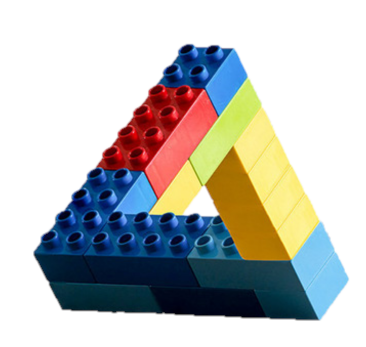
\includegraphics[scale=0.5]{img/penrose-triangle.eps}
 \captionsetup{labelformat=empty}
 \caption{彭罗斯三角形}
 \label{fig:Penrose-triangle}
\end{wrapfigure}

记得在中学数学课上,老师会在黑板上写一个充满字母的式子,然后让同学们化简。有同学会自告奋勇到讲台上拿起粉笔在黑板上推导。合并同类项、因式分解、各种办法都可以用。这个过程就像是变魔术,最后往往得到意想不到的简单结果。当然也有卡住或者绕圈子的时候,老师总是耐心地提示,引导我们找到思路。

这样的经历好像就发生在眼前,一方面,满手的粉笔灰让同学们体会到老师的不易,另一方面,那种推理的神秘强力量让我感到它的强大。我总是希望知道更多的公式,这样就能在化简或者推导时派上用场。

这种推理的神奇之处在于,我们不用特别关心这些公式或者定理在当时场景下的具体含义。就像摆动积木一样,从散落的各种零件,最后搭建起一个有趣玩具。这些公式和定理相互组装到一起,最后引向一个有趣的结果。看到$a^2 + 2ab + b^2$就会把它变换为$(a+b)^2$,就像把两块积木插到一起那样自然,我们不用在推理时强迫自己回想这个公式的几何意义。

\begin{figure}[htbp]
\centering
\begin{tikzpicture}
\draw[fill=gray, draw=black, pattern=north west lines]
  (0, 0) rectangle (4, 4);
\filldraw[fill=white]
  (0, 0) rectangle (1, 1)
  (1, 1) rectangle (4, 4);
\path (0.5, 0.5) node {$a^2$}
      (2.5, 2.5) node {$b^2$}
      (-0.5, 0.5) node {$a$}
      (2.5, 0.5) node {$ab$}
      (4.5, 2.5) node {$b$}
      (0.5, 2.5) node {$ab$};
\path (0, -1) node (l) {}
      (2, -1) node (m) {$a + b$}
      (4, -1) node (r) {};
\draw[->] (m) -- (l);
\draw[->] (m) -- (r);
\end{tikzpicture}
\caption{$(a + b)^2 = a^2 + 2ab + b^2$的几何意义}
\end{figure}

本章中,我们用两个例子说明如何进行编程中的推理。每个例子都首先用直观的方法给出分析和解释,然后再用纯推理的方式给出另一个解法。这就像$(a+b)^2$的情形。一方面我们可以用几何的直观,将其理解为一大一小两个小正方形和两个相等的矩形的面积;另一方面,我们也可以用纯推理一步一步导出同样的结果。

\[
\begin{array}{rcll}
(a + b)^2 & = & (a + b)(a + b) & \text{二次方的定义} \\
          & = & a(a + b) + b(a + b) & \text{乘法分配律} \\
          & = & a^2 + ab + ba + b^2 & \text{再次用分配律} \\
          & = & a^2 + 2ab + b^2 & \text{合并同类项$ab$和$ba$}
\end{array}
\]

\section{叠加——构建的融合}

我们要举的第一个例子是叠加——构建的融合(foldr/build fusion law)。2015年Java在其1.8版本中加入了lambda表达式并且提供了一系列支持函数式编程的工具。但是有人很快发现,尽管一连串地函数调用表达能力很强,简洁优雅,但是性能会下降很多。原因之一就是这些串起来函数调用产生了大量中间结果。这些中间结果往往不是一两个简单的数值,而通常是列表、容器这样规模很大的结构。这些结构被下一个函数消费使用,然后就丢弃了。但是接下来会产生另一个同等规模的结构。这种产生——一次性消费——丢弃——再产生的过程,沿着函数调用链一环一环地重复,造成了很大浪费。

例如\cite{GLPJ-1993},我们想判断一个列表中的每个元素是否都满足某个条件。可以这样定义:

\[
all(p, xs) = and(map(p, xs))
\]

传入$all(prime, [2, 3, 5, 7, 11, 13, 17, 19, ...])$就可以判断是否列表中都是素数。但是这个实现的效率却不高。首先$map(prime, xs)$会产生一个和$xs$同样长度的列表,列表中的每个元素是一个布尔值[True, True, ...],每个布尔值表示对应的元素是不是素数。然后这个布尔值列表传入$and$函数,检查是否存在False。最后$xs$和布尔值列表都被丢弃,而仅仅返回一个布尔值作为最终结果。

下面是另一种定义,它能够避免产生中间的布尔值列表:

\[
\begin{array}{l}
all(p, xs) = h(xs) \\
  \begin{cases}
  h([]) = True \\
  h(x:xs) = p(x) \land h(xs) \\
  \end{cases}
\end{array}
\]

虽然这个实现不产生中间结果,可是和前面的$and(map(p, xs)$比起来,既冗长又不直观。有没有什么办法,鱼和熊掌兼得,即不丧失直观性,又能避免低效的实现呢?我们发现有些变换满足这一要求。例如:

\[
map\ sqrt\  (map\ abs\ xs) = map\ (sqrt \circ abs) xs
\]

先把列表中每个元素取绝对值构成一列新数,然后再把这列数中的每个开方。这和把列表中每个数先取绝对值然后再立即开方后构成一列新数等价。由此我们可以得到一个转换规则:

\be
map\ f\ (map\ g\ xs) = map\ (f \circ g)\ xs
\ee

但是这样的规则太多了,我们无法全部把它们列出。并且在千变万化的程序中,我们无法一眼就看出应该用哪一条规则优化。吉尔(Gill)、朗奇布瑞(Launchbury)、佩顿琼斯(Peyton Jones)在1993年提出了一个方法,他们从列表最本质的构造和叠加操作入手,找到了优化的规律。

\subsection{列表的叠加操作}

我们在第一章就给出过列表的叠加操作,它的定义为:

\[
\begin{array}{l}
foldr\ \oplus\ z\ [] = z \\
foldr\ \oplus\ z\ (x:xs) = x\ \oplus\ (foldr\ \oplus\ z\ xs) \\
\end{array}
\]

展开就是:

\be
foldr\ \oplus\ z [x_1, x_2, ..., x_n] = x_1 \oplus (x_2 \oplus (...(x_n \oplus z))...)
\ee

许多列表相关的操作都可以用叠加来定义。我们接下来给出一些典型的例子:

\begin{enumerate}
\item 累加:

\[
sum = foldr\ +\ 0
\]

\item 前面提到的$and$函数,计算一个布尔值列表中的所有元素的逻辑与:

\[
and = foldr\ \land\ True
\]

这是因为:

\[
and\ [x_1, x_2, ..., x_n] = x_1 \land (x_2 \land (...(x_n \land True))...)
\]

\item 在一个列表中查找某一个元素是否存在:

\[
elem\ x\ xs\ = foldr\ (a\ b \mapsto a = x \lor b)\ False\ xs
\]

\item 逐一映射:

\[
\begin{array}{rcl}
map\ f\ xs & = & foldr\ (x\ ys \mapsto f(x) : ys)\ []\ xs \\
           & = & foldr\ ((:) \circ f)\ []\ xs \\
\end{array}
\]

\item 用某一条件过滤列表中的元素:

\[
\begin{array}{rl}
filter\ f\ xs = foldr\ (x\ ys \mapsto & if\ f(x)\ \\
                                      & then\ x:ys\ \\
                                      & else\ ys)\ []\ xs \\
\end{array}
\]

\item 两个列表连接:

\[
xs \doubleplus ys = foldr\ (:)\ ys\ xs
\label{eq:binary-concat}
\]

这是因为:

\[
[x_1, x_2, ..., x_n] \doubleplus ys = x_1 : (x_2 : (...(x_n : ys))...)
\]

\item 多个列表连接:

\[
concat\ xss = foldr\ \doubleplus\ []\ xss
\]

\end{enumerate}

叠加操作是如此基本,如果我们能把列表的叠加操作的化简规律找到,就找到了几乎所有列表操作的化简规律。

\subsection{叠加——构建融合律}
现在我们考虑,如果把空列表[](即Nil)和连接操作“:”(即Cons)进行叠加会产生什么结果。

\be
foldr\ (:)\ []\ [x_1, x_2, ..., x_n] = x_1 : (x_2 : (...(x_n : []))...)
\label{eq:foldr-fixed-point}
\ee

这回我们得到了列表本身。你也许想到了上一章介绍的不动点,我们稍后会回到这个话题。换言之,如果我们有一个运算$g$,它能够从一个起始值,例如[],和一个二元组合运算,例如“:”,产生一个列表。我们可以定义这个列表构造过程$build$:

\be
build(g) = g((:), [])
\label{eq:build-definition}
\ee

接着,如果用另一个起始值$z$和二元组合运算$f$,对这一列表进行叠加,其结果就相当于用$z$替换[],用“$f$”替换“(:)”,然后直接调用过程$g$。

\be
\pmb{foldr}(f, z, \pmb{build}(g)) = g(f, z)
\ee

写成无参数括号的形式就是:

\be
\pmb{foldr}\ f\ z\ (\pmb{build}\ g) = g\ f\ z
\label{eq:foldr-build-fusion-law}
\ee

我们称这一结果为\textbf{叠加——构建融合定律}。

在继续深入介绍前,让我们先看一些具体的例子。考虑如何计算从$a$到$b$间的整数和$sum([a, a+1, ..., b-1, b])$。为此我们可以先产生从$a$到$b$之间的所有整数$a, a+1, a+2, ..., b-1, b$,例如使用下面的方法:

\[
range(a, b) =
\begin{cases}
a > b: & [] \\
\text{否则}: & a : range(a+1, b) \\
\end{cases}
\]

这样$range(1, 5)$就产生列表[1, 2, 3, 4, 5]。现在我们只要把这个列表中的元素累加起来就得到答案了:

\[
sum(range(a, b))
\]

接下来关键的一步,我们把$range$中的起始值[]和二元组合运算(:)抽出成为参数:

\[
range'(a, b, \oplus, z) =
  \begin{cases}
  a > b: & z \\
  \text{否则}: & a \oplus range'(a+1, b, \oplus, z) \\
  \end{cases}
\]

我们甚至可以把$range'$的后两个参数克里化:

\[
range'\ a\ b = f\ c \mapsto
  \begin{cases}
  a > b: & c \\
  \text{否则}: & f\ a\ (range' (a+1)\ b\ f\ c) \\
  \end{cases}
\]

这样原来的$range$就可以用$range'$和$build$表示了:

\[
range(a, b) = build(range'(a, b))
\]

写下来我们用融合律化简累加和的计算:

\[
\begin{array}{rcll}
sum(range(a, b)) & = & sum(build(range'(a, b))) & \text{代入} \\
  & = & \pmb{foldr}\ (+)\ 0\ (\pmb{build}\ (range'\ a\ b)) & \text{用叠加表示累加} \\
  & = & range'\ a\ b\ (+)\ 0 & \text{使用融合律} \\
\end{array}
\]

这样就完成了化简,避免产生了中间列表。优化了算法。我们可以看一下最后算法的效果:

\[
range'\ a\ b\ (+)\ 0 =
  \begin{cases}
  a > b: & 0 \\
  \text{否则}: & a + range'(a+1, b, (+), 0) \\
  \end{cases}
\]

\subsection{列表的构建形式}

为了方便使用融合律,我们可以把常见的能够产生新列表操作都写为$build...foldr$的形式。这样当用叠加操作和这种形式的操作组合起来时,$\pmb{foldr}...(\pmb{build}...foldr)$,就可以使用融合律化简。

首先是最简单的操作——构造空列表:

\[
[] = build\ (f\ z \mapsto z)
\]

我们可以代入$build$的定义(\ref{eq:build-definition})来验证这个定义:

\begin{proof}
\bre
build\ (f\ z \mapsto z) & = & (f\ z \mapsto z)\ (:)\ [] & build\text{的定义} \\
  & = & (:)\ [] \mapsto [] & \beta-\text{规约,参见第二章} \\
  & = & [] & \\
\ere
\end{proof}

接下来是列表的链接(Cons)操作:

\[
x : xs = build\ (f\ z \mapsto f\ x\ (foldr\ f\ z\ xs))
\]

我们来验证一下:

\begin{proof}
\blre
  & build\ (f\ z \mapsto f\ x\ (foldr\ f\ z\ xs)) & \\
= & (f\ z \mapsto f\ x\ (foldr\ f\ z\ xs))\ (:)\ [] & build\text{的定义} \\
= & x : (foldr\ (:)\ []\ xs) & \beta-\text{规约} \\
= & x : xs & \text{由(\ref{eq:foldr-fixed-point}),叠加的不动点} \\
\elre
\end{proof}

然后是列表的连接:

\[
xs \doubleplus ys = build\ (f\ z \mapsto foldr\ f\ (foldr\ f\ z\ ys)\ xs)
\]

\begin{proof}
\blre
  & build\ (f\ z \mapsto foldr\ f\ (foldr\ f\ z\ ys) xs) & \\
= & (f\ z \mapsto foldr\ f\ (foldr\ f\ z\ ys)\ xs)\ (:)\ [] & build \text{的定义} \\
= & foldr\ (:)\ (foldr\ (:)\ []\ ys)\ xs & \beta-\text{规约} \\
= & foldr\ (:)\ ys\ xs & \text{对内层用叠加的不动点} \\
= & xs \doubleplus ys & \text{由(\ref{eq:binary-concat}),列表的连接} \\
\elre
\end{proof}

以下操作我们只列出结果,我们把它们的证明作为本小节的练习。
多个列表的连接:

\[
concat\ xss = build\ (f\ z \mapsto foldr\ (xs\ x \mapsto foldr\ f\ x xs)\ xss)
\]

一一映射产生新列表:

\[
map\ f\ xs = build\ (\oplus\ z \mapsto foldr\ (y\ ys \mapsto (f\ y) \oplus ys)\ z\ xs)
\]

过滤元素产生新列表:

\[
filter\ f\ xs = build\ (\oplus\ z \mapsto foldr\ (x\ xs' \mapsto
  \begin{cases}
    f(x): & x \oplus xs' \\
    \text{否则}: & xs' \\
  \end{cases})\ z\ xs) \\
\]

重复不断产生同一元素的(无穷)列表:

\[
repeat\ x = build\ (\oplus\ z \mapsto let\ r = x \oplus r\ in\ r)
\]

\subsection{使用融合律化简}

\subsection{类型限制}

\subsection{用范畴论推导融合律}

\begin{Exercise}
\Question{验证从左侧叠加也可以表示为$foldr$:
\[
foldl\ f\ z\ xs = foldr\ (b\ g\ a \mapsto g\ (f\ a\ b))\ id\ xs\ z
\]}
\Question{证明以下列表的构建——叠加形式:
\[
\begin{array}{l}
concat\ xss = build\ (f\ z \mapsto foldr\ (xs\ x \mapsto foldr\ f\ x xs)\ xss) \\
map\ f\ xs = build\ (\oplus\ z \mapsto foldr\ (y\ ys \mapsto (f\ y) \oplus ys)\ z\ xs) \\
filter\ f\ xs = build\ (\oplus\ z \mapsto foldr\ (x\ xs' \mapsto
  \begin{cases}
    f(x): & x \oplus xs' \\
    \text{否则}: & xs' \\
  \end{cases})\ z\ xs) \\
repeat\ x = build\ (\oplus\ z \mapsto let\ r = x \oplus r\ in\ r) \\
\end{array}
\]
}
\end{Exercise}

\section{KMP匹配算法}

我们给出的第二个例子是著名的KMP字符串匹配算法。

\cite{Bird-2010} pp. 117-135

\ifx\wholebook\relax \else
\begin{thebibliography}{99}

\bibitem{GLPJ-1993}
Andrew Gill, John Launchbury, Simon L. Peyton Jones. ``A Short Cut to Deforestation''. Functional programming languages and computer architecture. pp. 223-232. 1993.

\bibitem{Bird-2010}
Richard Bird. ``Pearls of Functional Algorithm Design''. Cambridge University Press; 1 edition November 1, 2010. ISBN: 978-0521513388.

\end{thebibliography}

\expandafter\enddocument
%\end{document}

\fi
